\section{Linear Model for Classification}

As said in the previous lecture, a simple linear model, represents an hyperplane. In dimension $D$, we can write:
\begin{align*} 
	y = w^{\left(0\right)} + w^{\left(1\right)}x^{\left(1\right)} + \cdots + w^{\left(D\right)}x^{\left(D\right)} = w^{T}\begin{pmatrix} 1 \\ x^{\left(1\right)} \\ x^{\left(2\right)} \\ \vdots \\ x^{\left(D\right)} \end{pmatrix} 
\end{align*}
Ultimately, whatever the input dimension, we can write:
\begin{align*} 
	y = w^{T}x
\end{align*}
with $x \in \mathbb{R}^{D + 1}$, where the extra dimension contains a $1$ to account for $w^{\left(0\right)}$.
\subsection{Loss Function ad Empricial Risk}
\begin{framedremark}
Those are general machine learning concept
\end{framedremark}
\begin{parag}{Loss function}
    \begin{definition}
    The loss function $l\left(\hat{y}_i, y_i\right)$ computes an error value between the prediction and the true value
    \end{definition}
	This is a general machine learning conecpt, this is not used only for linear regression, we will see different loss functions in the upcoming lectures.
\end{parag}
$ $\\
The goal of the loss function is to \important{measure} how \important{wrong} our prediction is. Meaning that if we were to train a model in order to guess wether it is a dog, cat, ship, plane, etc.. The loss function will tell us how wrong are we. (notice that even with classification model we will need to have a loss function (even is it will measure a 'yes' or 'no' type question)).

\begin{center}
    

\begin{tikzpicture}[
	scale=0.2,
  font=\sffamily,
  >=Latex,
  box/.style={draw, rounded corners=16pt, very thick,
              minimum width=3.2cm, minimum height=2.2cm, align=center},
  lab/.style={align=center},
]

% --- Left: training images (stack) ---
\node (img1) {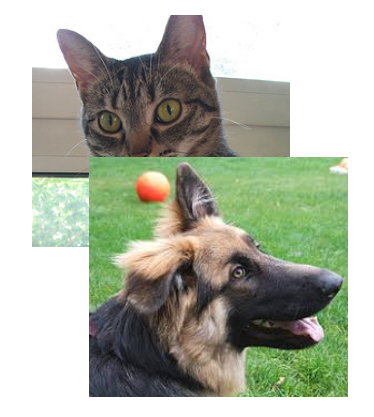
\includegraphics[width=1.55cm]{screenshots/2026-03-04.png}};
\node[below=6mm of img2] (vdotsL) {\Large$\vdots$};
\node[below=8mm of vdotsL] (img3) {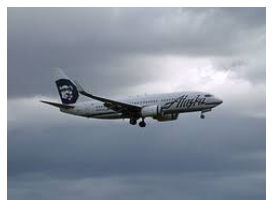
\includegraphics[width=1.95cm]{screenshots/2026-03-04_1.png}};

\node[lab, below=10mm of img3] (trainlab) {\Large Training\\images};

% Arrow into model
\draw[->, very thick] ($(img2.east)+(6mm,0)$) -- ++(100mm,0);

% --- Center: model box ---
\node[box, right=22mm of img2] (model)
{\Large Model\\[2mm]\large (trainable parameters)};

% Arrow out of model
\draw[->, very thick] (model.east) -- ++(80mm,0);

% --- Predicted labels (left label column) ---
\node[right=35mm of model.center, yshift=12mm] (p1) {\Large Cat};
\node[below=5mm of p1] (p2) {\Large Cat};
\node[below=11mm of p2] (pvd) {\Large$\vdots$};
\node[below=11mm of pvd] (p3) {\Large Ship};

\node[lab, below=16mm of p3] {\Large Predicted\\labels};

% --- True labels (right label column) ---
\node[right=42mm of p1] (t1) {\Large Cat};
\node[below=5mm of t1] (t2) {\Large Dog};
\node[below=11mm of t2] (tvd) {\Large$\vdots$};

% --- Loss arrow between predicted and true labels ---
\draw[<->, very thick]
  ($(pvd.east)+(5mm,0)$) -- node[midway, above=1mm, font=\Large\itshape]{Loss}
  ($(tvd.west)+(-5mm,0)$);

% Ellipses near the loss arrow ends (as in the figure)
\node at ($(pvd.east)+(2mm,0)$) {\Large :};
\node at ($(tvd.west)+(-2mm,0)$) {\Large :};

% --- Optional: far-right "plot/image" block (bottom-right) ---
\node[right=22mm of tvd, yshift=-22mm] (plot)
{\includegraphics[width=2.25cm]{lossplot.jpg}};

\end{tikzpicture}
\end{center}

\begin{parag}{Loss function: Examples}
    So far, we have already seen quite a lot of loss functions for linear regression:
	\begin{itemize}
	    \item Single ouput dimension: $l\left(\hat{y}_i, y_i\right) = \left(\hat{y}_i - y_i\right)^2$
	    \item Multiple output dimension: $l\left(\hat{y}_i, y_i\right) = || \hat{y}_i - y_i||^2$
	\end{itemize}
	In principle, other loss function could be used for regression, for example, using the MAE evaluation metric
	\begin{align*} 
	l\left(\hat{y}_i, y_i\right) = \left\|\hat{y}_i - y_i\right\|
	\end{align*}
	As we will see later today and in future lectures, other loss function can be used for classification.
\end{parag}

\begin{parag}{Empirical risk}
	\begin{definition}{Empirical Risk}
		$ $\\
    Given $N$ training sample $\left\{\left(x_i, y_i\right)\right\}$, the empirical risk is defined as:
	\begin{align*} 
		R\left( \{x_i\}, \{y_i\}, w\right) = \frac{1}{N}\sum_{i = 1}^{N}l\left(\hat{y}_i , y_i\right)
	\end{align*}
	Where $\left\{x_i\right\}$, and $\left\{y_i\right\}$ are the sets of training inputs and labels, respectively.
	\end{definition}
	When we are training our model, the goal is to minimize the empirical risk --  find the parameters $w$ (e.g., $w^{\left(0\right)}, w^{\left(1\right)}$) that minimize the empirical risk.
	\begin{subparag}{Remark}
	    Note that the risk depends on $w$ via $\hat{y}_i $.
	\end{subparag}
\end{parag}
\begin{parag}{Minimzing the risk}
    This is expressed as the optimization problem:
	\begin{align*} 
		\min_w \frac{1}{N}\sum_{i= 1}^{N}l\left(\hat{y}_i , y_i\right)
	\end{align*}
	We can also write that the best parameters as a solution to the following equation:
	\begin{align*} 
		w^{\ast}  = \text{argmin}_w \frac{1}{N}\sum_{i = 1}^{N}l\left(\hat{y}_i , y_i\right)
	\end{align*}
	This is what we have done when training our linear regressor. Our least-square minimization problem is one example of empirical risk minimization, using the square loss.
\end{parag}
\begin{parag}{From regression to classification}
    As said before, how we created classification model was directly based from a regression task. We took our training data and label, and mapped them into A $D + 1$ dimension. For instance given data point x with $x^{\left(1\right)}$ and $x^{\left(2\right)}$ and two calsses $0$ and $1$, we would ouput our data as:
	\begin{center}
	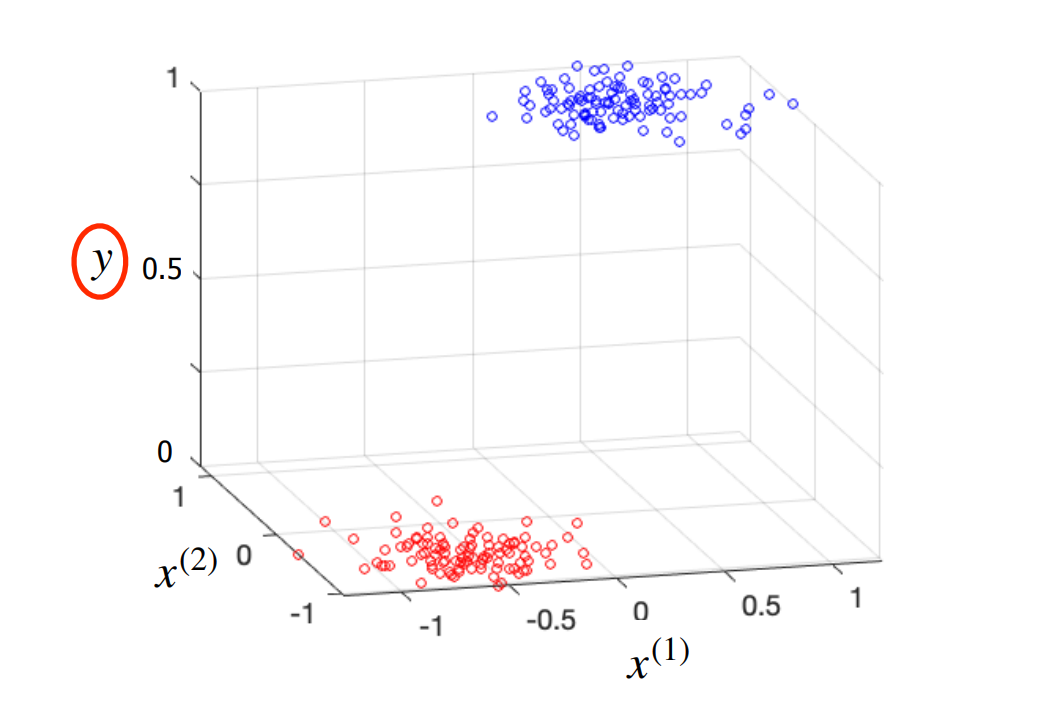
\includegraphics[scale=0.2]{screenshots/2026-02-24_2.png}
	\end{center}
	Then we would train our regression model with our data which will give us a plane:

	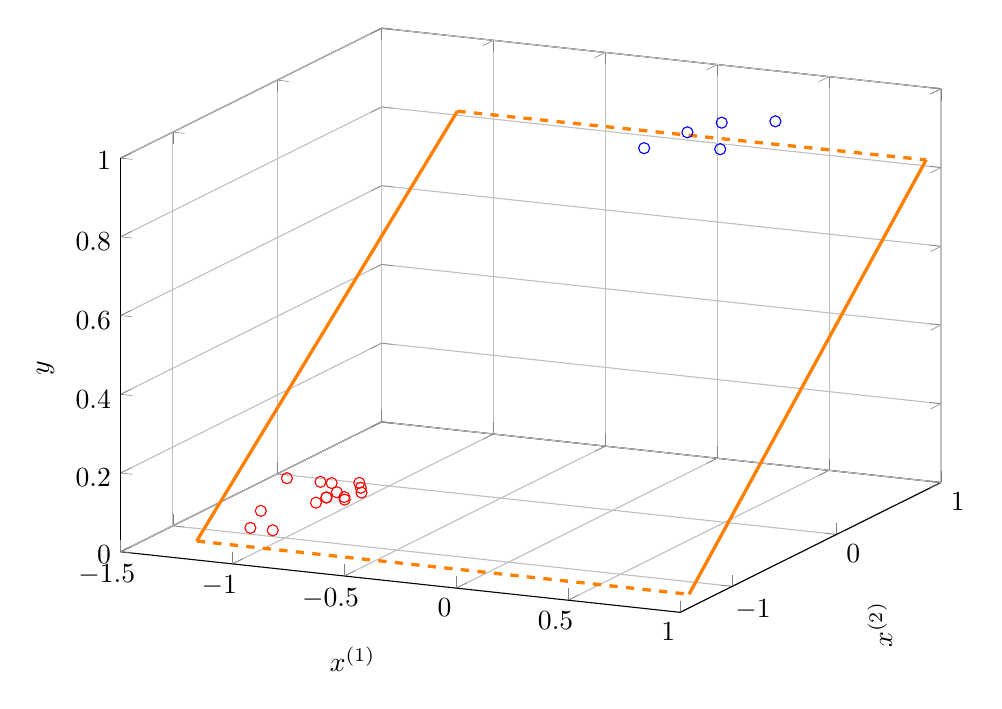
\begin{tikzpicture}
\begin{axis}[
    view={25}{20},
    axis lines=box,
    xmin=-1.5, xmax=1,
    ymin=-1.5, ymax=1,
    zmin=0, zmax=1,
    xlabel={$x^{(1)}$},
    ylabel={$x^{(2)}$},
    zlabel={$y$},
    grid=major,
    width=12cm,
    height=9cm,
]

% --- Blue class (top points) ---
\addplot3[
    only marks,
    mark=o,
    blue,
] table {
0.1 0.5 0.9
0.2 0.6 0.85
0.3 0.4 0.95
0.0 0.3 0.88
0.4 0.7 0.92
};

% --- Red class (bottom points) ---
\addplot3[
    only marks,
    mark=o,
    red,
] table {
-1.0 -0.6 0.05
-1.0 -0.7 0.05
-1.0 -0.5 0.05
-1.0 -0.6 0.05
-0.8 -0.7 0.10
-1.1 -0.9 0.00
-1.2 -0.9 0.00
-0.9 -0.5 0.08
-1.00 -0.55 0.08
-1.05 -0.55 0.08
-1.20 -0.55 0.08
-0.83 -0.79 0.08
-0.85 -0.75 0.08
-0.82 -0.65 0.08
-1.2 -0.8 0.03
};


% Choose two points A and B in the (x,y) base, then extend to z=1
\coordinate (A)  at (axis cs:-1.30,-1.20,0);
\coordinate (B)  at (axis cs: 0.90,-1.20,0);
\coordinate (Ap) at (axis cs:0.90,-3.42,1.52);
\coordinate (Bp) at (axis cs: 1.47,-0.15,1);

% solid sides
\draw[orange, very thick] (A) -- (Ap);
\draw[orange, very thick] (B) -- (Bp);

% dashed top & bottom
\draw[orange, very thick, dashed] (A) -- (B);
\draw[orange, very thick, dashed] (Ap) -- (Bp);
\end{axis}
\end{tikzpicture}

The linear model encodes the plan that passes through the samples (orange plane). To turn this into a classification model, we need to find the \important{decision boundary}
\begin{framedremark}
I just want to emphasize what is going on here. 
We first try to model the data using a linear model of the form 
\[
f(x)=w^Tx+b .
\]
The parameters of this model are chosen to minimize a certain 
\important{loss function}, which measures how well the model fits the training data.
\\
$ $\\
After this, the goal is to create a classification model from the model we just built.
In binary classification, the decision boundary is defined by
\[
w^Tx+b=0 .
\]
In general, for data in $D$ dimensions, this equation defines a 
$(D-1)$ -dimensional hyperplane. In particular, when $D=2$, the decision 
boundary is a straight line.
\end{framedremark}
\end{parag}



\begin{parag}{Adding non-linearity}
    The output of the linear model $w^{T}x$ is a continuous value. However classification model output a label (a discrete value). We therefore need to '\textit{cast}' our value before output:
	\begin{align*} 
		y = \begin{cases}
			1 \text{ if } w^{T}x \geq 0.5\\
			0 \text{ otherwise}
		\end{cases}
	\end{align*}
\end{parag}
\begin{parag}{Step function: Drawback}
    However the gradient of the step function is not continuous, this means that using gradient descent won't work very well, optimizing become pretty hard.

	\begin{subparag}{Remark}
		The perceptron algorithm can nonetheless handle the two-class case, but we will not cover it in this course.
	\end{subparag}
	The better way is to use a '\textit{smoother}' step function: the logistic sigmoid function:
	\begin{align*} 
		f\left(a\right) = \frac{1}{1 + \exp(-a)}
	\end{align*}
	\begin{center}
	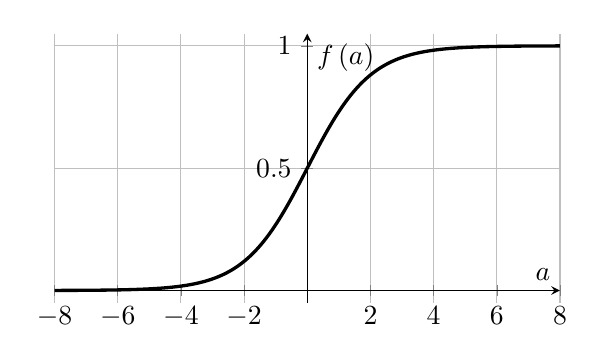
\begin{tikzpicture}
\begin{axis}[
    width=8cm,
    height=5cm,
    xmin=-8, xmax=8,
    ymin=-0.05, ymax=1.05,
    axis lines=middle,
    xlabel={$a$},
    ylabel={$f\left(a\right)$},
    grid=major,
    samples=300,
    domain=-8:8,
    ytick={0,0.5,1},
]
\addplot[very thick] {1/(1+exp(-x))};
\end{axis}
\end{tikzpicture}
	\end{center}
	With a 1 $D$ input $x$, applying the logistic function to the output of a linear model gives a prediction:
	\begin{align*} \hat{y} = \frac{1}{1 + \exp\left(-w^{\left(0\right)} - w^{\left(1\right)}x\right)} \end{align*}
	Now an interesting thing to see is the effect of each parameters on our $\hat{y}$:
	\begin{center}
	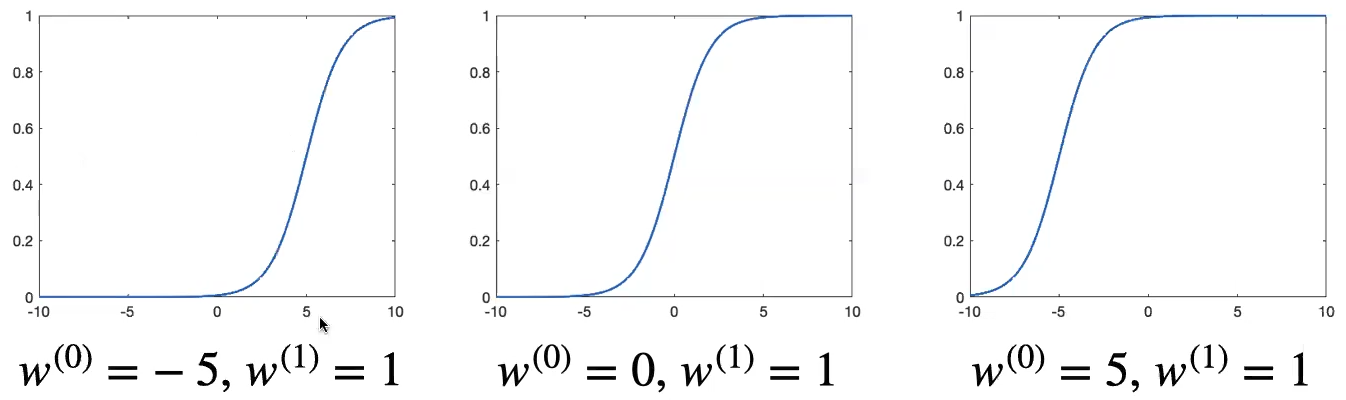
\includegraphics[scale=0.2]{screenshots/2026-02-26_2.png}
	\end{center}
\end{parag}

\begin{parag}{Probabilistic interpretation}
    In the binary case, with $D$ dimensional inputs, we can write the prediction of the model as:
	\begin{align*} 
		\hat{y} =  \sigma\left(w^{T}x\right) = \frac{1}{1 + \exp\left(-w^{T}x\right)}
	\end{align*}
	Such a prediction can be interpreted as the probability that $x$ belongs to the positive class (or as a score for the positive class). The probability to belong the negative class is then computedd as $1 - \hat{y}$.
\end{parag}
\begin{parag}{Logistic regression}
    \begin{definition}
    The model whose prediction is defined as 
	\begin{align*} 
		\hat{y} = \sigma\left(w^{T}x\right) x = \frac{1}{1 + \exp\left(-w^{T}x\right)}
	\end{align*}
	Is call a \important{logistic regression}
    \end{definition}
	\begin{subparag}{Remark}
	    Note that this name is slightly misleading, as this is truly a classification model, not a regression one
	\end{subparag}
	At its heart, logistic regression still use a linear model, but followed by a non-linearity to better encore the underlying binary classification problem.
\end{parag}
\begin{parag}{Logistic regression: Training}
    Given $N$ training samples, to learn the parameters $w$ of the logistic regression model, we need to define a loss function. Instead of using the $L_2$ loss as in the least-square case, this is achieved by making use of the probabilistic interpreation.
	\begin{subparag}{Remark}
	    \begin{itemize}
			\item Because knowledge of probabilities is not required for this course, the derivation of the loss function that follows will be a bit hand-wavy
			\item Nevertheless, this loss remains intuitive: The loss is such that it aimes to find the parameters that maximize the probability of the correct class for each training sample
	    \end{itemize}
	\end{subparag}
	Specifically, the logistic regression loss is derived by first writing the following likelihood estimator:
	\begin{align*} 
	p\left(y | w\right) = \prod_{i = 1}^{N} \hat{y}_i^{y_i} \cdot \left(1 - \hat{y}_i \right)^{1 - y_i}
	\end{align*}
	Because, a product of terms between 0 and 1 can be unstable to optimize, we take the logarithm of this likelihood and take its negative to define an empricial risk to minimize, written as 
	\begin{align*} 
		R\left(w\right) =  -\sum_{i = 1}^{N}\left(y_i \ln\left(\hat{y}_i \right) + \left(1 - y_i\right)\ln\left(1 - \hat{y}_i \right)\right)
	\end{align*}
	This loss function is known as the cross-entropy (AICC II mentionned?)
\end{parag}
Since $y_i$ is either $0$ or $1$, the cross-entropy can be re-written as:
\begin{align*} 
	R\left(w\right) = \sum_{i \in \text{positive samples}} \ln\left(\hat{y}_i \right) - \sum_{i \in \text{negative sample}} \ln\left(1 - \hat{y}_i \right)
\end{align*}
A very nice thing here for us is that, the \important{cross-entropy is a convex function}. But in this case, its minimization as no closed-form solution. This means that we will need to use an approximation: \important{gradient descent}!!

\begin{figure}[h!]
    \centering
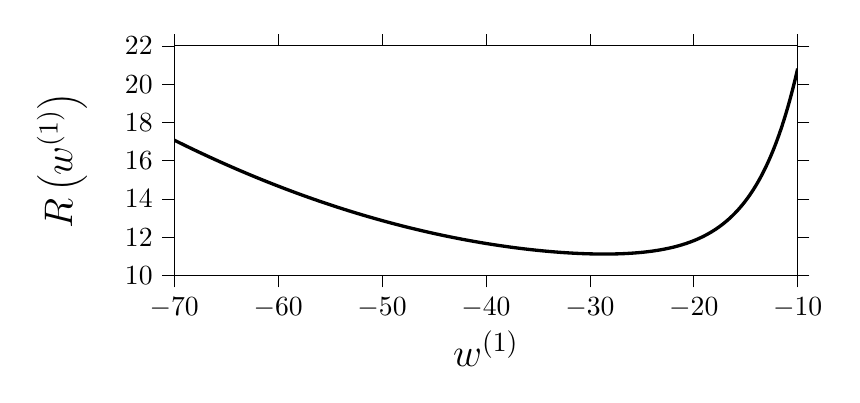
\begin{tikzpicture}
\begin{axis}[
    width=9.5cm,
    height=4.5cm,
    xmin=-70, xmax=-10,
    ymin=10, ymax=22,
    xtick={-70,-60,-50,-40,-30,-20,-10},
    ytick={10,12,14,16,18,20,22},
    axis lines=box,
    tick align=outside,
    tick style={black},
    xlabel={$w^{(1)}$},
    xlabel style={font=\Large, yshift=2pt},
    ylabel={$R\left(w^{(1)}\right)$},
    ylabel style={
        font=\Large,
        rotate=0,
        at={(axis description cs:-0.18,0.50)},
        anchor=center
    },
    grid=none,
    samples=400,
    domain=-70:-10,
]

% A convex "risk-like" curve shaped like the course screenshot
% minimum near -25, steep rise near -10
\addplot[very thick] {11 + 0.003*(x+25)^2 + 0.75*exp(0.25*(x+20))};

\end{axis}
\end{tikzpicture}
\caption{Cross entropy}
\end{figure}
\begin{parag}{Probabilistic Derivation}
    As we have now all did probability and statistics, we can still build it ourself. First, for us to train our model via the maximum likelihood estimator, we need to understand from where it comes from. We will do it as follow:
	\begin{itemize}
		\item Choosing a probabilistic model for $y | x$
		\item Writing the likelihood of the observed labels
		\item Maximizing it (equivalently minimizing the negative log-likelihood)
	\end{itemize}
	First, in logistic regression we have $\theta = \left(w, b\right)$.	Where $w \in \mathbb{R}^{D}$ are the weights and $b$ is the bias. (we can also see $\theta \in \mathbb{R}^{D + 1}$).\\
	$ $\\
	Secondly, logistic regression assumes a probability model for the labels. For each data point $x$ we have that:
	\begin{align*} 
		P\left(Y = 1 | x, \theta\right) =  \sigma\left(\theta^{T}x\right)
	\end{align*}
	What this says to us: given $x$, the label $y$ folows a \important{bernoulli distribution}:
	\begin{align*} 
		Y | x \sim \text{bernoulli}\left(\sigma\left(\theta^{T}x\right)\right)
	\end{align*}
	Then given that we can compute the likelihood estimator as we used to. First defined it:
	\begin{align*} 
		\mathcal{L}\left(\theta\right) &= P\left(y_1, y_2, \ldots, y_n| x_1, x_2, \ldots, x_n, \theta\right)\\
									   &= \prod_{i = 1}^{n}P\left(y_i | x_i, \theta\right)
	\end{align*}
	If we develop this we get:
	\begin{align*} 
		\mathcal{L}\left(\theta\right) =  \prod_{i = 1}^{n} \sigma\left(\theta^{T}x_i\right)^{y_i}\left(1 - \sigma\left(\theta^{T}x_i\right)\right)^{1 - y_i}
	\end{align*}
	Now that we have defined it we seek to find the $\theta^{\ast}$ such that:
	\begin{align*} 
		\theta^{\ast} = \text{arg} \max_\theta \mathcal{L}\left(\theta\right)
	\end{align*}
	And as we did in statistics, we can take the log of this function and computing the maximum on the log which is '\textit{nicer}'. We therefore try to maximize:
	\begin{align*} 
		\sum_{i= 1}^{n}\left(y_i\log \sigma\left(\theta^{T}x_i\right) + \left(1 - y_i\right)\log \left(1 - \sigma\left(\theta^{T}x_i\right)\right)\right)
	\end{align*}
	\begin{subparag}{Intuition}
	    \begin{itemize}
			\item The data already exists
			\item We assume a \important{probabilistic model}
			\item The model has parameter $\theta$
			\item We ask:
				\begin{center}
				    For which $\theta$ would this observed data be the most likely
				\end{center}
	    \end{itemize}
	    
	\end{subparag}
	
\end{parag}



\subsection{Iterative, Gradient-based optimization}
\begin{parag}{Minimizing a function}
    With 1D function for which the soltuon cannot be computed in closed form, one can nonetheless use the derivative
	\begin{itemize}
		\item Recall that it represents the slope at a given point, and thus indicates in which direction to move to reach a lower function value
	\end{itemize}
	Therefore the algorithm can be define pretty easily:
	\begin{enumerate}
	    \item Initialize $w_0$ (randomly)
	    \item While not converged do 
			\begin{enumerate}
			    \item Update $w_k \leftarrow w_{k-1} - \nu \frac{d T\left(w_{k-1}\right)}{dw}$
			\end{enumerate}
	\end{enumerate}
	The $\nu$ defines the step size of each iteration. (often called the learning rate)
\end{parag}
\begin{parag}{Convergence criteria}
    This is nice but we still need so potential convergence criteria to be sure that our algorithm works effectively:
	\begin{itemize}
	\item Change in function values less than threshold: $\left\|R\left(w_{k-1} - R\left(w_k\right)\right)\right\| < \delta_R$
	\item Change in parameter value less than threshold: $\left\|w_{k-1} - w_k\right\| < \delta_w$
	\item Maximum number of iterations reached, Meaning that we have no guarantee to have reached the minimum
	\end{itemize}
	\begin{framedremark}
	In theory, one would need the function to has lipschitz continuous gradient  in order to have stable steps. What this means is we will assume:
	\begin{align*} 
		|| \nabla R\left(x\right) - \nabla R\left(y\right)|| \leq L||x - y||
	\end{align*}
	The rule mentionned above are more practical criteria. In practie we don't want to compute exact optimality, we so care more about:
	\begin{itemize}
		\item change in objective
		\item change in parameters
	\end{itemize}
	These word well \important{because} the function is convex + smooth
	\end{framedremark}
	When minimizing we have to be carefule about:
	\begin{subparag}{Influence of $\nu$}
	    Too large steps can lead our algorithm to start jumping around the 'solution' and oscillate till infinity. We are not able to have a magic formula to have a good $\eta$, each $\eta$ is problem-dependent.
	\end{subparag}
	\begin{subparag}{Influence of the initial $w_0$}
		Assuming that our function is convex, the algorithm will always converges to the same point. Choosing a good $w_0$ will still converge to the same point, but \important{faster}.
	\end{subparag}
\end{parag}
\begin{parag}{Minimizing a non-convex function}
    As in convex function, we can still use the same iterative algorithm as before. However this time. The output of our algorithm depends now on $w_0$. we can now be stuck at local minimum and at saddle point.
	\begin{subparag}{Remark}
	    Note that this is problem-dependent and the values used here are very different from those used in the convex sample before.
	\end{subparag}
	In practice, we have more than one parameter, i.e. $w \in \mathbb{R}^{D + 1}$, and we thus use the function gradient:
	\begin{align*} 
		\nabla_w R\left(w\right) = \begin{pmatrix} \frac{\partial R}{\partial w^{\left(0\right)}}  \\ \frac{\partial R}{\partial w^{\left(1\right)}}  \\ \frac{\partial R}{\partial w^{\left(2\right)}}  \\ \vdots \\ \frac{\partial R}{\partial w^{\left(D\right)}}  \end{pmatrix} 
	\end{align*}
	Where $\frac{\partial R}{\partial w^{\left(j\right)}} $ denotes the partial derivative w.r.t. variable $w^{\left(j\right)}$
\end{parag}
\begin{parag}{Recap: Properties of gradient}
	\begin{itemize}
    The gradient at a point $w$ has the direction of greatest increase of the function at $w$
    \item Its magnitude is the rate of increase in that direction
\end{itemize}
\end{parag}
\begin{parag}{Gradient descent on multivariate function}
    The algorithm stays the same but we will use the gradient instead:
	\begin{enumerate}
	    \item Initialize $w_0$ (e.g., randomly)
	    \item While not converged:
			\begin{enumerate}
			\item Update $w_k \leftarrow w_{k-1} - \eta \nabla_W R\left(w_{k-1}\right)$
			\end{enumerate}
	\end{enumerate}
	The learning rate $\eta$ has the same effect as in the 1D case.\\
	$ $\\
	Convergence can again be measured by:
	\begin{itemize}
	    \item Thresholding the change in function value
	    \item Thresholding the change in paramters, e.g. $||w_{j-1} - w_k|| < \delta_w$
	\end{itemize}
\end{parag}
\begin{parag}{Minmizing a non-convex function \\ Example: Sine- and Cosine based function of 2 variables}
	Let our function be:
	\begin{align*} 
		R\left(w\right) = \sin\left(w^{\left(0\right)}\right) + \cos\left(w^{\left(1\right)}\right)
	\end{align*}
\end{parag}

\begin{center}
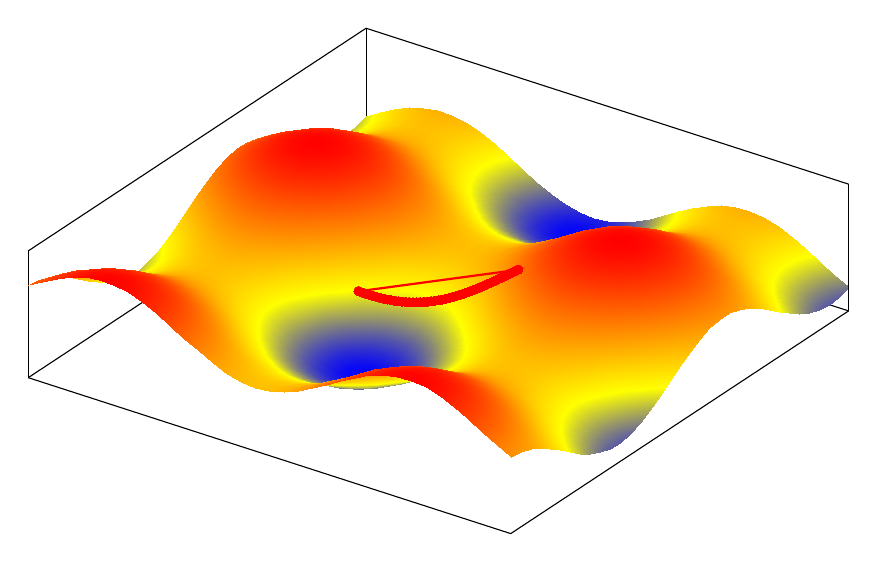
\begin{tikzpicture}
\begin{axis}[
    view={35}{65},
    axis lines=box,
    xmin=0, xmax=10,
    ymin=0, ymax=10,
    zmin=-2.2, zmax=2.2,
    ticks=none,
    width=12cm,
    height=8cm,
]

% Surface: R(w)=sin(w0)+cos(w1)
% (PGFPlots trig uses degrees, so wrap with deg(.))
\addplot3[
    surf,
    samples=35,
    samples y=35,
    domain=0:10,
    y domain=0:10,
    shader=interp,
    mesh/ordering=y varies,
] {sin(deg(x)) + cos(deg(y))};

% Red trajectory curve drawn on the surface (illustrative path)
\addplot3[
     thick,
    red,
    mark=*,
    mark size=1.2pt,
    samples=45,
    domain=-6:6,
] ({5 + 0.22*x},
   {5 + 0.08*x},
   {sin(deg(5 + 0.22*x)) + cos(deg(5 + 0.08*x))});

\end{axis}
\end{tikzpicture}

\end{center}
As in the 1D cases the same issues can arise:
\begin{itemize}
	\item Different learning reate can yield different results
	\item Different Initializations can yield different results
\end{itemize}

\begin{parag}{Back to Logistic Regression}
    With binary ground-truth label $y_i$, the corss entropy can be written as:
	\begin{align*} 
		R\left(w\right) &= \sum_{i \in \text{positive samples}} \ln\left(\hat{y}_i \right) - \sum_{i \in \text{negative sample}} \ln\left(1 - \hat{y}_i \right)\\
						&= \sum_{i \in \text{positive samples}} \ln \sigma\left(w^{T}x_i\right) - \sum_{i \in \text{negative sample}} \ln\left(1 - \sigma\left(w^{T}x_i\right)\right)\\
	\end{align*}
	To minimize it via gradient descent, we need to compute its gradient. Using the chain rule, and after some derivation, we have:
	\begin{align*} 
		\nabla_w\left(-\sum_{i \in \text{positive}} \ln \sigma \left(w^{T}x_i\right)\right) = \sum_{i \in \text{positive}} \left(\hat{y}_i - 1\right)x_i =  \sum_{ i \in \text{positive}} \left(\hat{y}_i  - y_i\right)x_i
	\end{align*}
	Similarly, for the negative examples, we have:
	\begin{align*} 
		\nabla_w \left(- \sum_{i \in \text{negative}}\ln \left(1 - \sigma\left(w^{T}x\right)\right)\right) =  \sum_{i \in \text{negative}} \hat{y}_i x_i =  \sum_{i \in \text{negative}}\left(\hat{y}_i  - y_i\right)x_i
	\end{align*}
	Finally,this can be put back together to obtain:
	\begin{align*} 
		\nabla_w R\left(w\right) =  \sum_{i = 1}^{N} \left(\hat{y}_i  - y_i\right)x_i
	\end{align*}
	Where $y_i$ is the true label for sample $i$, i.e. 1 for positive sample and 0 for negative samples\\
	$ $\\
	Intuitively, the gradient is given by the error of the current prediction $\left(\hat{y}_i - y_i\right)$, multiplied by the input.
\end{parag}
\begin{parag}{Example}
    If we take the previous example and compare the least-square classification (in green) and the logistic regression in magenta, we get:
	\begin{center}
	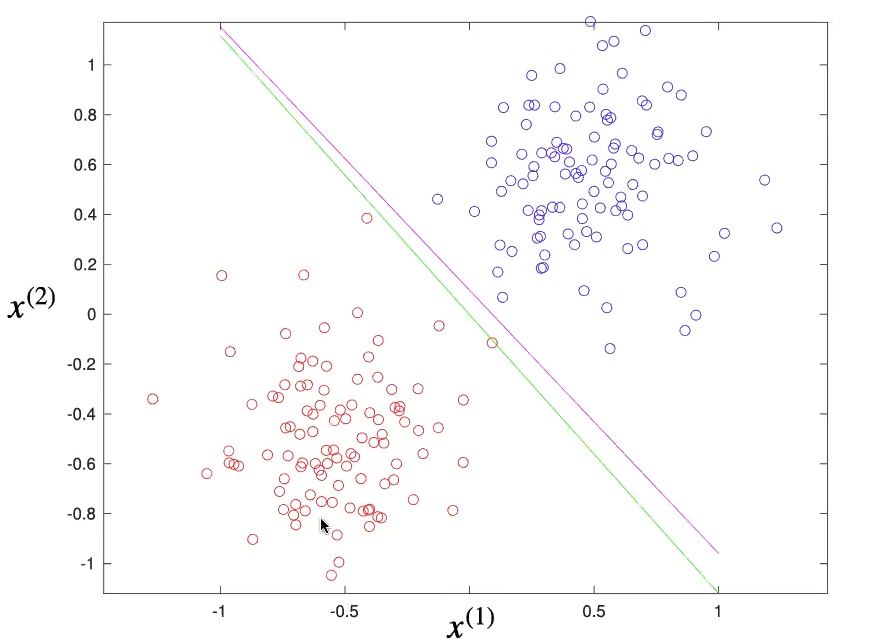
\includegraphics[scale=0.2]{screenshots/2026-02-26_5.png}
	\end{center}
	But now, with additional samples, the boundary remains correct:
	\begin{center}
	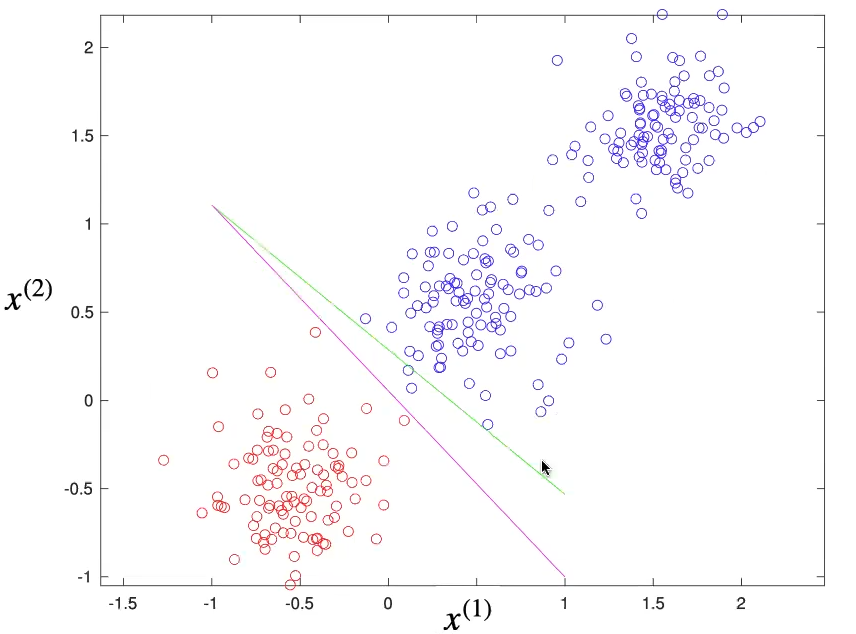
\includegraphics[scale=0.2]{screenshots/2026-02-26_6.png}
	\end{center}
\end{parag}
\begin{framedremark}
	As with linear regression, the learned coefficients of logistic regression can also be analyzed, see a discussion of this at \href{https://www.displayr.com/how-to-interpret-logistic-regression-coefficients/}{\url{https://www.displayr.com/how-to-interpret-logistic-regression-coefficients/}} (this is not part of the course)
\end{framedremark}
\begin{parag}{Linear models}
    The real difference between these models is the loss function.
	\begin{itemize}
		\item The choise of loss function has an impact on the resulting algorithm
		\item Let's have a look at the intuition behind SVM
	\end{itemize}
\end{parag}
\begin{parag}{Margin}
	To have a better intuition of the SVM we first need to introduce the notion of \important{margin}:
	\begin{definition}
	The distance between the decition boundary and the nearest sample is called \important{margin}
	\end{definition}

\end{parag}
	\begin{figure}[h!]
	\centering
	
\includegraphics[width=0.4\textwidth]{figure/2026-02-26}
	\caption{margin}
	\end{figure}
	Intuitively, a good decision boundary should maximize the margin. Such a boundary is determined by a subset of the data points, named support vectors (indicated with circles) when we have two classes what this essentially means is that our boundary will be centered between both our classes.

\begin{parag}{Support Vector Machine}
    The SVM classifier is a binary classifier based on the linear model as before:
	\begin{align*} 
		\hat{y} = w^{T}x
	\end{align*}
	It aims to maximize the margin while enforcing a correct classification for each training samples. This is formulated as a convex optimization problem that can be solved to optimality with standard iterative solvers\\
	$ $\\
	In the presence of additional samples, the decision boundary is unchanged. The goal of this model is not to have a '\textit{weighted mean}' it's more finding the \important{best boundary} such that the score is minimize. The only vector that truly matter are the one close to the decision boundary.
\end{parag}
\begin{parag}{Loss function}
    Ultimately, training an SVM can be written as:
	\begin{align*} \min_{w^{(0)}, \widetilde{w}} \frac{1}{2C}\|\widetilde{w}\|^2
+ \sum_{i=1}^{N}\max\left(0, 1 - y_i \left(w^{(0)} + \widetilde{w}^Tx_i\right)\right)
	\end{align*}
	\begin{itemize}
	    \item The term $\mid\mid\widetilde{w}\mid\mid^2$ corresponds to the inverse of the margin (distance between the decision boundary and the nearest sample); minimizing it seeks to maximize the margin
	    \item The term:
			\begin{align*} 
				\max\left(0, 1 - y_i\left(w^{\left(0\right)} + \widetilde{w}^{T}x_i\right)\right)
			\end{align*}
			is referred to as the \important{hinge loss} and encourages correctly classifying each sample.
	\end{itemize}
	
\end{parag}















